\section{Spectroscopic Completeness} \label{sec:spec_comp}
Spectroscopic galaxy surveys, such as BGS, do not successfully measure the
redshift for all of the galaxies they target. 
As a result, this spectroscopic incompleteness must be accounted for when
measuring galaxy population statistics such as the SMF.  
In this appendix, we present how we estimate the spectroscopic incompleteness
for BGS and derive the weights we use to correct for its impact on the SMF. 

For BGS, spectroscopic incompleteness is primarily driven by fiber assignment
and redshift failures.  
DESI uses 10 fiber-fed spectrographs with 5000 fibers but targets more galaxies
than available fibers. 
For instance, the BGS Bright and Faint samples have $\sim 860$ and 
$530\,{\rm targets}/{\rm deg}^2$, respectively. 
For the 8 ${\rm deg}^2$ field-of-view of DESI, this roughly correspond to
11,000 targets, significantly more than the 5000 available fibers. 
DESI only measures the spectra of targets that are assigned fibers. 
In fact, of the 5000, a minimum of 400 ‘sky’ fibers are dedicated to measuring
the sky background for accurate sky subtraction and an additional 100 fibers
are assigned to standard stars for flux calibration~\cite{guy2022}.

Furthermore, each fiber is controlled by a robotic fiber positioner on the
focal plane. 
These positioners can rotate on two arms and be positioned within a circular
patrol region of radius 1.48 arcmin~\citep{schubnell2016, desi2016a,2022b, silber2022}.
Although the patrol regions of adjacent positioners slightly overlap, the
geometry of the positioners cause higher incompleteness in regions with high
target density~\citep{smith2019}.
To mitigate the incompleteness from the fiber assignment, BGS will observe its  
footprint with four passes.
With this strategy, BGS achieves $\sim$80\% fiber assignment
completeness~\citep{hahn_bgs}.

To estimate fiber assignment completeness, we run the fiber assignment
algorithm~\citep{raichoor2022} on BGS targets 128 separate times.
For each BGS galaxy, $i$, we count the total number of times out of 128 that
the galaxy is assigned a fiber: $N_{i, {\rm FA}}$. 
Then to correct for the fiber assignment incompleteness, we assign correction
weights
\begin{equation} \label{eq:w_fa}
    w_{i, \mathrm{FA}} = \frac{128}{N_{i, \mathrm{FA}}}
\end{equation}
to each BGS galaxy. 
{\color{red} explain what this means} 

\begin{figure}[h]
\begin{center}
    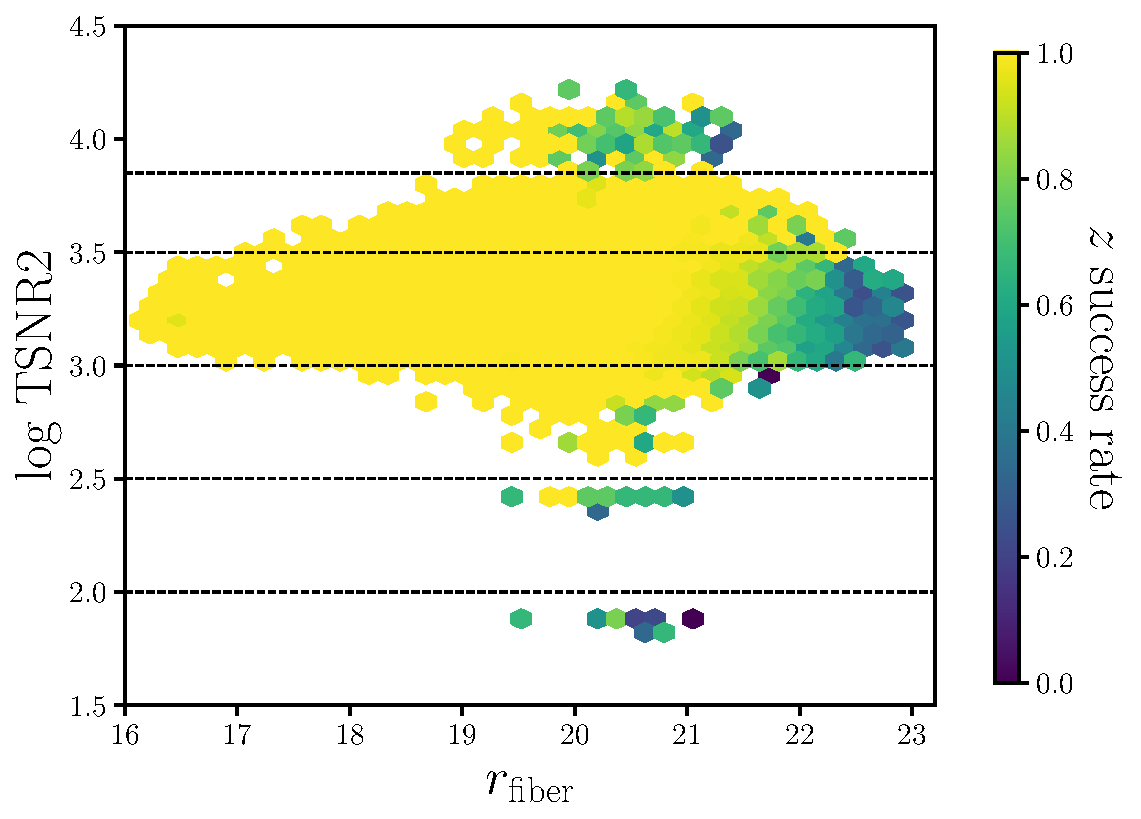
\includegraphics[width=0.5\textwidth]{figs/bgs_bright_rfib_tsnr2.pdf} 
    \caption{
        Redsift success rate of BGS Bright galaxies as a function of 
        $r_{\rm fiber}$ and TSNR2.
        TSNR2 is a statistic that quantifies the signal-to-noise ratio of the
        observed spectrum. 
        The color map represents the mean redshift success rate in each hexbin.
        We mark the TSNR2 bins (black dashed) that we use to separately fit the
        redshift success rate as a function of $r_{\rm fiber}$ using
        Eq.~\ref{eq:zsucc}.
        In each TSNR2 bin, redshift success decreases as $r_{\rm fiber}$
        increases. 
    }\label{fig:zfail0}
\end{center}
\end{figure}

Although we measure a spectrum for each galaxy assigned a fiber, we do not
accurately measure redshifts for every spectra. 
This redshift measurement failure significantly contributes to spectroscopic
incompleteness. 
For BGS, redshift failure of an observed galaxy spectrum depends mainly on
fiber magnitude and a statistic, TSNR2.
Fiber magnitude is the predicted flux of the BGS object within a 1.5\arcsec
diameter fiber; we use $r$-band fiber magnitude, $r_{\rm fiber}$.  
TSNR2 roughly corresponds to the signal-to-noise ratio of the spectrum and is 
the statistic used to calibrate the effective exposure times in DESI
observations (\todo{CITE}).

In Figure~\ref{fig:zfail0}, we present the redshift, $z$, success rate of BGS
Bright galaxies as a function of $r_{\rm fiber}$ and TSNR2.
In each hexbin, the color map represents the mean $z$-success rate. 
We include all hexbins with more than 2 galaxies. 
Overall, the $z$-success rate depends significantly on $r_{\rm fiber}$:
galaxies with fainter $r_{\rm fiber}$ have lower $z$-success rates. 
However, the $r_{\rm fiber}$ dependence itself varies in bins of TSNR2. 
We mark the edges of the bins in black dashed: $\log {\rm TSNR2} = 2.0, 2.5,
3.0, 3.5, 3.85$.
Within each of the TSNR2 bins, the $r_{\rm fiber}$ dependence of the
$z$-success rate does not vary significantly. 
In Figure~\ref{fig:zfail1}, we present the $z$-success rate of BGS Bright
galaxies as a function of $r_{\rm fiber}$ for each of the 6 TSNR2 bins.
We mark the range of TSNR2 in the bottom left of each panel. 
The errorbars represent the Poisson uncertainties of the $z$-success rate.

\begin{figure}
\begin{center}
    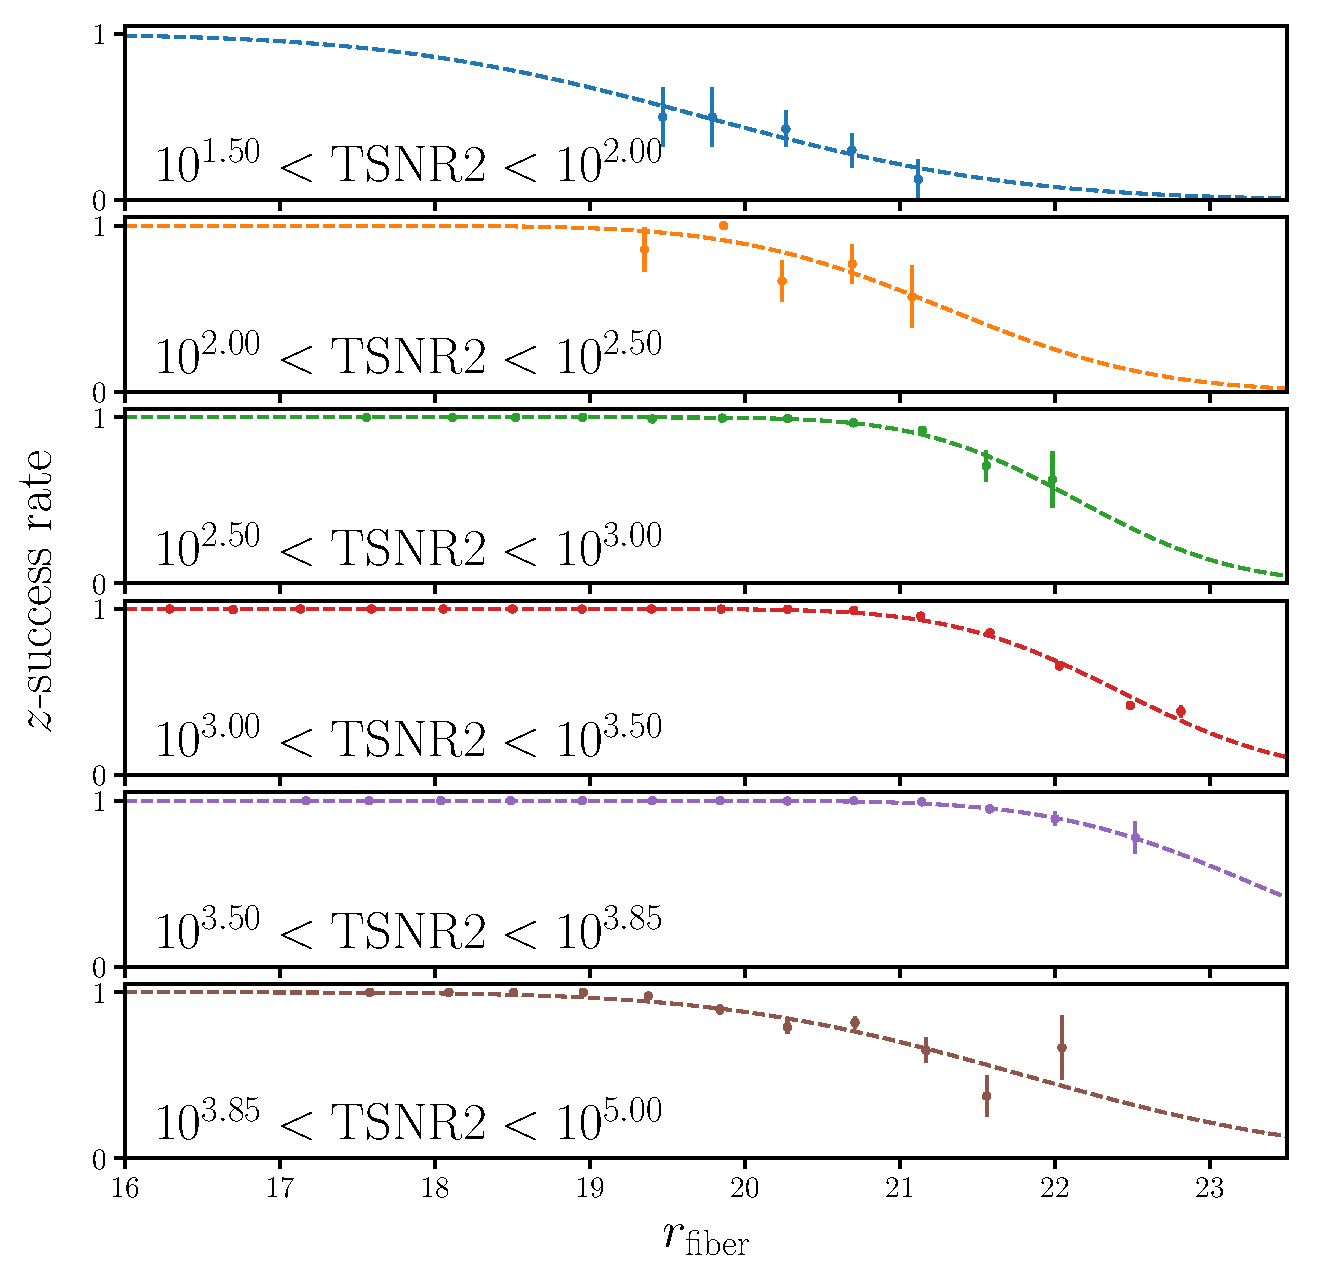
\includegraphics[width=0.5\textwidth]{figs/bgs_bright_rfib_tsnr2_zsuccess.pdf}
    \caption{
        Redshift success rates of BGS Bright galaxies  as a function of 
        $r_{\rm fiber}$ in 6 TSNR2 bins. 
        The error bars represent the poisson uncertainties.
        In each panel, we include the best-fit analytic (Eq.~\ref{eq:zsucc})
        approximation of the redshift success rate (dashed) derived from
        $\chi^2$ minimization. 
        We use this analytic approximation to calculate the galaxy weights to
        correct for spectroscopic incompleteness caused by failures to
        accurately measure redshifts from observed spectra.
    }\label{fig:zfail1}
\end{center}
\end{figure}

To correct for the effect of redshift failures, we include an additional
correction weight for each BGS galaxy: 
\begin{equation}
    w_{i, {\rm ZF}} = \frac{1}{f_{z-{\rm sucess}}(r_{{\rm fiber},i}, {\rm
    TSNR2}_i)}.
\end{equation} 
$f_{z-{\rm sucess}}(r_{{\rm fiber},i}, {\rm TSNR2}_i)$ is the $z$-success rate
as a function of $r_{\rm fiber}$ and TSNR2 of the galaxy. 
Galaxies with $f_(z-{\rm sucess} = 1.$ (100\% $z$-success) will have 
$w_{i, {\rm ZF}} = 1$ while galaxies with $f_(z-{\rm sucess} = 0.1$ 
(10\% $z$-success) will have $w_{i, {\rm ZF}} = 10$.
For $f_{z-{\rm sucess}}(r_{{\rm fiber},i}, {\rm TSNR2}_i)$, we fit the
following functional form for each TSNR2 bin: 
\begin{equation} \label{eq:zsucc}
    f_{z-{\rm success}}(r_{\rm fiber}) = \frac{1}{2} \bigg(1-{\rm erf}(c_0
    (r_{\rm fiber} - c_1))\bigg).
\end{equation}
In Figure~\ref{fig:zfail1}, we present the best-fit 
$f_{z-{\rm success}}(r_{\rm fiber})$ for each of the TSNR2 bins in dashed. 
The best-fit coefficients, $c_0, c_1$, are derived from $\chi^2$ minimization.
We list the best-fit values for each TSNR2 bin in Table~\ref{tab:zfail}. 

\begin{table} 
    \caption{Best-fit coefficients of the $z$-success rate as a function of
    $r_{\rm fiber}$ for different TSNR2 bins.} 
    \begin{center}
        \begin{tabular}{lcc} \toprule
            TSNR2 range & $c_0$ & $c_1$ \\[3pt]
            \hline 
            $10^{1.5}   - 10^{2}$       & 0.443 & 19.7 \\ 
            $10^{2}     - 10^{2.5}$       & 0.668 & 21.3 \\ 
            $10^{2.5}   - 10^{3}$       & 0.888 & 22.1 \\ 
            $10^{3}     - 10^{3.5}$       & 0.822 & 22.4 \\ 
            $10^{3.5}   - 10^{3.85}$    & 0.698 & 23.3 \\ 
            $10^{3.85}  - 10^{5}$      & 0.465 & 21.8 \\ 
            \hline            
\end{tabular} \label{tab:zfail}
\end{center}
\end{table}

% --- references ---
% https://desi.lbl.gov/trac/wiki/ClusteringWG/LSScat/DA02main/current_version#clusteringfiles
